\documentclass[preprint,12pt]{elsarticle}
% Robotics and Autonomous Systems (Elsevier) -- manuscript source.
% Editor-ready project generated by make_latex_project.py from manuscripts/main.tex.
% Sections in sections/, figures in figures/, tables in tables/, Supplementary in supplementary/.

\usepackage{amsmath,amssymb}
\usepackage{graphicx}
\usepackage{booktabs,multirow,array}
\usepackage[hidelinks]{hyperref}
\usepackage{lineno}
\usepackage{xcolor}
\graphicspath{{figures/}}
\newcommand{\tabdir}{tables/}
\renewcommand{\Pr}{\operatorname{P}}
\newcommand{\Bin}{\operatorname{Bin}}
\linenumbers

\journal{Robotics and Autonomous Systems}

\begin{document}

\begin{frontmatter}

\title{When Recovery Hurts: Separating Rescue from Harm in an Observation-Only Recovery Intervention for a Frozen Visuomotor Policy}

% AUTHOR ITEMS TO CONFIRM: name spelling, affiliation, e-mail, ORCID (see editorial/author_items_to_confirm.md)
\author[1]{[Author name to confirm]}
\ead{[corresponding e-mail to confirm]}
\affiliation[1]{organization={[Affiliation to confirm]},
            country={[Country to confirm]}}

\begin{abstract}
Recovery interventions on frozen robot policies are usually judged by the failures they repair, but the same intervention can also turn an episode the policy would have completed into a failure, and a net success gain hides that effect. We study this for a diffusion policy stacking cubes in simulation. When the policy is about to open its gripper over the target, an observation-only controller (Vision-CENTER V2) estimates the horizontal offset between the two cubes from a base and a wrist RGB camera and a short visual memory, and either abstains or makes a bounded horizontal move; the policy's action queue is then cleared and the policy re-plans. Each scene is branched from one simulator snapshot, so intervened and uninterrupted runs are paired, and rescues (failure to success) and harms (success to failure) are counted separately. After development, two pre-registered confirmatory stages used new scenes. On 400 calibration scenes per policy, harm was 1 of 348 and 0 of 337 baseline successes; exact binomial tests with Holm correction rejected a conditional harm rate of 5\% or more for both policies (family-wise error $\delta=0.05$). On 400 held-out test scenes per policy, run once, success rose from 350 to 379 and from 347 to 373 (29 rescues vs 0 harms, $p=1.9\times10^{-9}$; 27 vs 1, $p=1.1\times10^{-7}$). Much of the harm margin comes from scenes in which the controller abstains. We also report a failed contact-measurement check. The certificate is statistical and task-level, not a physical safety guarantee.
\end{abstract}

\begin{keyword}
recovery intervention \sep frozen visuomotor policy \sep paired evaluation \sep outcome harm \sep finite-sample certificate \sep diffusion policy \sep robotic manipulation
\end{keyword}




\end{frontmatter}

%% ---------------------------------------------------------------------------------------------------------
\section{Introduction}\label{sec:intro}

Learned visuomotor policies such as diffusion policies \cite{chi2023diffusion} are increasingly deployed as frozen components: after training, their weights are fixed, and any further improvement must come from outside the network. A natural outside improvement is a runtime recovery intervention: a rule or monitor decides that something is about to go wrong, a small controller changes the state, and the policy resumes. Many methods of this kind exist, from learned recovery policies \cite{reichlin2022manifold,cideron2023getback,vats2025recoverychaining} to human or learned interventions during interactive imitation \cite{ross2011dagger,kelly2019hgdagger,hoque2022thrifty}, and runtime monitors that detect or predict failures \cite{agia2025unpacking,romer2025fiper,liu2023reflect,duan2025aha}.

\paragraph{Why harm must be measured separately}
An intervention on a frozen policy changes the state from which the policy continues. If the policy would have failed, the change can rescue the episode. If the policy would have succeeded, the same change can cause a failure, for example by spending part of the time budget or by leaving the gripper in a configuration from which the policy does not recover. On $n$ paired scenes with $R$ rescues and $H$ harms, the change in success rate is
\begin{equation}\label{eq:delta}
\Delta_{\mathrm{succ}} \;=\; \frac{R-H}{n}.
\end{equation}
Two interventions with $(R,H)=(30,0)$ and $(60,30)$ have the same $\Delta_{\mathrm{succ}}$, but the second loses 30 episodes that the user could previously rely on. A success rate, or a comparison of success rates measured on different scenes, cannot distinguish them; only a paired comparison on the same states can. Harm therefore needs its own measurement and, if an intervention is to be deployed on top of a policy that already works most of the time, its own bound.

\begin{figure}[!htbp]
\centering
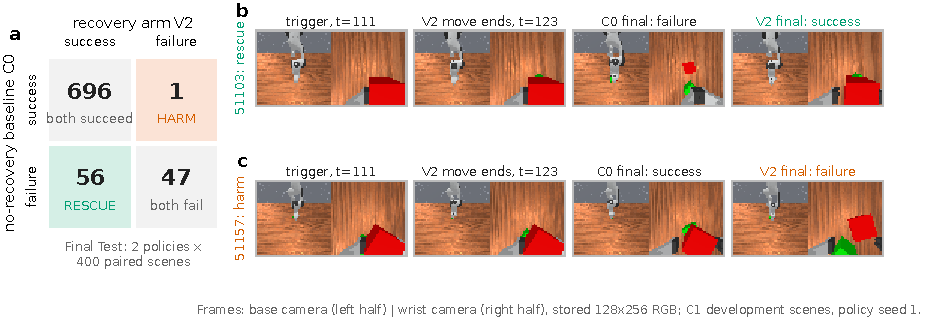
\includegraphics[width=\linewidth]{Fig01_problem_rescue_vs_harm.pdf}
\caption{Rescue and harm. (a) Paired outcome matrix of the Final Test, pooled over the two policies (descriptive; the tests are per policy). (b) A development rescue (scene 51103, policy seed 1; the first seed-1 rescue in scene order): the policy alone fails; after the V2 move the re-planned policy places the cube and the episode succeeds. (c) The only development harm of V2 for policy seed 1 (scene 51157): the policy alone drops the cube beside the target, regrasps it and succeeds at step 190; with V2 the episode fails. Each frame is the stored base-camera (left half) and wrist-camera (right half) RGB image, without processing or overlay.}\label{fig:problem}
\end{figure}

\paragraph{Detection is not intervention}
A failure monitor answers whether something will go wrong; it does not answer whether a particular action taken at that moment will make the outcome better or worse. The second question is counterfactual: it compares the outcome with and without the action from the same state \cite{ahmedt2026rescue}. In this paper the trigger is a fixed, observable rule, so the object of study is the intervention itself, not the detector.

\paragraph{Case study}
We study one intervention in depth: an observation-only, gated centring move at the moment a frozen diffusion policy is about to release a cube over another cube. We chose it because it can be evaluated cleanly: it acts at most once per episode, it uses only the robot's cameras and proprioception, it needs no retraining, and when it abstains the episode is exactly the uninterrupted one. The question we answer is: \emph{can such an intervention increase task success while keeping, with a finite-sample statistical guarantee, the rate at which it turns the policy's own successes into failures below a stated level?} We answer it for one task, one intervention and two independently trained policies, and we report every step of the argument, including the parts that did not work.

The study rests on three design choices.
\begin{enumerate}
\item \textbf{Paired branching.} Each scene runs once until the trigger; the simulator state is saved, and the uninterrupted policy (C0), the proposed controller and all ablations are run from that same snapshot. Each scene yields a pair of outcomes $(Y_0, Y_g)$ and falls into one of four cells: both succeed, rescue, harm, both fail (Fig.~\ref{fig:problem}a).
\item \textbf{Harm as a conditional rate.} We define harm as $h(g)=\Pr(Y_g=0 \mid Y_0=1)$, the probability that intervention $g$ turns a baseline success into a failure, and test $h(g)<\varepsilon$ against $h(g)\ge\varepsilon$ with an exact binomial test on calibration scenes that were not used for development.
\item \textbf{Separation of certificate and efficacy.} The harm certificate is computed on a calibration split; the efficacy claim (more successes than without the intervention) is tested once on a separate, held-out test split, under a frozen and hashed protocol. Development results motivate the design and are reported as such.
\end{enumerate}

\paragraph{The strongest objection, stated first}
A low harm rate can simply mean that the controller rarely acts. This is largely true here: V2 abstains in about four of five triggered scenes, and harm can only occur in scenes where it moves. Restricted to the baseline successes in which it moved, the observed harm is 1 of 48 and 0 of 36 on calibration, and the corresponding one-sided upper bounds are near 10\%, not 5\% (Section~\ref{sec:confirm}). We therefore state the certificate as a property of the deployed system, the policy together with its gated controller, and we do not claim that the abstention rules themselves reduce harm: an ablation without the V2-specific rules rescued slightly more scenes without additional harm in development (Section~\ref{sec:discussion}).

\paragraph{Contributions}
\begin{itemize}
\item A paired evaluation protocol for recovery interventions on a frozen policy that reports rescue and harm separately, certifies the conditional harm rate with a pre-registered exact test on a calibration split, and confirms efficacy once on a held-out split (Sections~\ref{sec:problem} and~\ref{sec:protocol}).
\item Vision-CENTER V2, an observation-only release-time centring controller with a confirmed visual memory and explicit abstention rules, described as implemented (Section~\ref{sec:method}).
\item A two-stage confirmatory result on 1,600 new paired scenes for two policies (Section~\ref{sec:confirm}).
\item A descriptive mechanism analysis that follows a representative rescue and the single development harm through observation, memory, decision, movement and hand-back, with a commanded-versus-actual motion audit of all development moves (Section~\ref{sec:mechanism}).
\item An audit of the physical record used by that analysis, including a pre-declared check that fails, a partial explanation of the failure, and a statement of what it does and does not affect (Section~\ref{sec:physics}).
\end{itemize}

We do not claim physical safety, transfer to other tasks or to a real robot, or novelty of paired counterfactual evaluation, of exact binomial bounds or of risk control; these are established tools \cite{clopper1934,holm1979,angelopoulos2021ltt,ahmedt2026rescue}. The contribution is their combination for a runtime recovery intervention, with a calibration/test separation and a code-level account of why the intervention rescues and how it harms. The controller is task-specific; we present it as a case study of the protocol, which is the part we expect to transfer.

%% ---------------------------------------------------------------------------------------------------------
\section{Related work}\label{sec:related}

\paragraph{Recovery for learned policies}
Learned policies drift away from the states seen in demonstrations, and the resulting compounding error is the classical motivation for interactive imitation learning \cite{ross2011dagger,laskey2017dart}. Recovery methods return the system to familiar states: Back to the Manifold learns to steer out-of-distribution states back to the data manifold \cite{reichlin2022manifold}, POIR plans a return to the demonstration distribution \cite{cideron2023getback}, RecoveryChaining learns local recovery policies that hand control back to a nominal controller \cite{vats2025recoverychaining}, and Recovery RL restricts exploration with a learned recovery policy \cite{thananjeyan2021recoveryrl}. Recent work on vision--language--action and world--action models adds recovery at scale \cite{liufu2026repovla,li2026causalhistory}, retries after failure \cite{du2024toerr}, or rewinds to an earlier state \cite{zheng2026rewind}. These methods are usually evaluated by success rate with and without recovery; our concern is the decomposition of that difference into rescues and harms on paired states.

\paragraph{Interventions and runtime monitoring}
Interactive imitation learning lets a human or a gate decide when to intervene \cite{kelly2019hgdagger,hoque2022thrifty}. Runtime monitors detect failures of generative policies from consistency and progress \cite{agia2025unpacking} or predict them online \cite{romer2025fiper}; language-model systems explain and correct failures \cite{liu2023reflect,duan2025aha}; CheckVLA verifies action chunks with a world model \cite{liu2026checkvla}. A failure prediction does not say whether acting on it helps. RESCUE makes exactly this point and evaluates monitor alarms by counterfactual interventions from the same policy state \cite{ahmedt2026rescue}, and a recent study audits whether memory in history-conditioned policies actually guides decisions \cite{zhang2026memory}. Our evaluation shares the counterfactual, same-state view; it adds a pre-registered confirmatory split and a certificate on the harm side.

\paragraph{Statistical risk control}
Learn then Test calibrates algorithms so that a chosen risk is controlled with finite-sample guarantees through multiple testing \cite{angelopoulos2021ltt}. Our certificate is the simplest instance of this idea: a single, pre-specified candidate and one binomial test per policy, combined with Holm's procedure \cite{holm1979}. The efficacy test is the exact one-sided form of McNemar's paired test \cite{mcnemar1947}.

Table~\ref{tab:related} positions the present work against the closest papers. The table describes what each paper evaluates as stated in that paper; it is not a ranking.

\begin{table}[!htbp]
\centering\footnotesize
\caption{Positioning against related work (qualitative; based on each paper's own description).}\label{tab:related}
\begin{tabular}{p{0.24\linewidth}p{0.30\linewidth}p{0.38\linewidth}}
\toprule
Work & Primary question & Difference from this paper\\
\midrule
DAgger, DART, HG-DAgger, ThriftyDAgger \cite{ross2011dagger,laskey2017dart,kelly2019hgdagger,hoque2022thrifty} & collect corrective data or gate human interventions during training & the policy here is frozen; interventions are evaluated, not used for training\\
Back to the Manifold, POIR, RecoveryChaining, Recovery RL \cite{reichlin2022manifold,cideron2023getback,vats2025recoverychaining,thananjeyan2021recoveryrl} & learn a recovery behaviour & our controller is hand-designed and bounded; we separate its rescues from its harms on paired states\\
Sentinel, FIPER, REFLECT, AHA, CheckVLA \cite{agia2025unpacking,romer2025fiper,liu2023reflect,duan2025aha,liu2026checkvla} & detect, predict or explain failures & we evaluate what an action taken at the trigger does to the outcome\\
RESCUE \cite{ahmedt2026rescue} & is an alarm worth acting on? counterfactual interventions from the same state & we add a calibration certificate for harm and a held-out confirmatory test\\
To Err is Robotic, Rewind-IL, RePO-VLA, Causal-History TTS \cite{du2024toerr,zheng2026rewind,liufu2026repovla,li2026causalhistory} & retry, rewind or optimise for recovery & we report conditional harm on baseline successes, not only success rate\\
Learn then Test \cite{angelopoulos2021ltt} & finite-sample risk control by multiple testing & we apply its simplest form to harm of one frozen candidate\\
\bottomrule
\end{tabular}
\end{table}


%% ---------------------------------------------------------------------------------------------------------
\section{Problem formulation}\label{sec:problem}

\paragraph{Research question} Given a frozen policy $\pi$ and an intervention $g$ that may act once per episode, does $g$ increase the success probability, and is the probability that it destroys a success of $\pi$ below $\varepsilon$?

\paragraph{Paired outcomes} A scene $s$ is drawn from a scene distribution $\mathcal{D}$: in the simulator, a scene seed determines the initial cube placement and the policy's sampling noise. The policy runs from the initial state until a trigger step $t^\star(s)$, determined by an observable rule (Section~\ref{sec:method}). The full simulator state and the policy state at $t^\star$ are saved. From that snapshot we run the policy unchanged, which gives $Y_0(s)\in\{0,1\}$, and the policy with intervention $g$, which gives $Y_g(s)\in\{0,1\}$. Scenes without a trigger, and scenes in which $g$ abstains, have $Y_g=Y_0$ by construction. The four cells are
\begin{equation}
\begin{aligned}
\text{rescue}: &\ Y_0=0,\ Y_g=1, & \qquad \text{harm}: &\ Y_0=1,\ Y_g=0,\\
\text{both succeed}: &\ Y_0=1,\ Y_g=1, & \qquad \text{both fail}: &\ Y_0=0,\ Y_g=0,
\end{aligned}
\end{equation}
and the success difference is Eq.~\eqref{eq:delta}.

\paragraph{Conditional harm} We define
\begin{equation}
h(g) \;=\; \Pr_{s\sim\mathcal{D}}\bigl(Y_g(s)=0 \,\bigm|\, Y_0(s)=1\bigr).
\end{equation}
It is the probability that a success the policy would have achieved alone is lost when $g$ is deployed. It concerns the task outcome in the simulator; it does not measure collision, force or damage.

\paragraph{Harm certificate} Let $n$ calibration scenes be drawn independently from $\mathcal{D}$. This is an assumption about the simulator's seed-to-scene map: distinct seeds are treated as independent draws of placement and noise, which a placement check supports but cannot prove (Supplementary Section~S1). Let $n_+=\sum_s Y_0(s)$ and $k=\sum_s Y_0(s)\,(1-Y_g(s))$. Conditional on which scenes have $Y_0=1$, those scenes are an i.i.d.\ sample from $\mathcal{D}$ given $Y_0=1$, so $k\sim\Bin(n_+, h(g))$. For the null hypothesis $H_0^{\mathrm{harm}}: h(g)\ge\varepsilon$ the exact p-value is
\begin{equation}\label{eq:cert}
p_{\mathrm{harm}} \;=\; \Pr\bigl(\Bin(n_+,\varepsilon)\le k\bigr) \;=\; \sum_{j=0}^{k}\binom{n_+}{j}\,\varepsilon^{j}(1-\varepsilon)^{n_+-j},
\end{equation}
which is valid because the binomial distribution function decreases in $h$. For the two policies we apply Holm's procedure \cite{holm1979} at family-wise level $\delta$: sort the two p-values, compare the smaller with $\delta/2$ and, if it is rejected, the larger with $\delta$. A policy is \emph{certified} when its null is rejected. The guarantee is frequentist: if $h(g)\ge\varepsilon$ for some policy in the family, the probability that the procedure nevertheless certifies that policy is at most $\delta$. It is not a statement that the true rate of a particular deployment is below $\varepsilon$ with probability $1-\delta$, and it holds only under the sampling assumption above and for the simulator configuration in which the calibration scenes were run. We pre-registered $\varepsilon=\delta=0.05$.

\paragraph{Efficacy test} On the held-out test scenes, let $b$ be the number of rescues and $c$ the number of harms. Under the null hypothesis that the intervention does not increase success, $\Pr(Y_0=0,Y_g=1)\le\Pr(Y_0=1,Y_g=0)$, and conditional on the $d=b+c$ discordant scenes the number of rescues is stochastically at most $\Bin(d,1/2)$. The exact one-sided p-value is
\begin{equation}\label{eq:eff}
p_{\mathrm{eff}} \;=\; \Pr\bigl(\Bin(d,1/2)\ge b\bigr) \;=\; \sum_{j=b}^{d}\binom{d}{j}2^{-d},
\end{equation}
the exact form of McNemar's paired test \cite{mcnemar1947}. Holm's procedure is applied over the two policies at $\alpha=0.05$. The unit of analysis is the scene; the two policies are tested separately, and pooled counts are descriptive only.

\paragraph{Information constraint} The trigger and the controller may use only the robot's cameras, its proprioception, the policy's own commands and their own history. They may not read object poses, grasp flags, the success flag or any future quantity from the simulator. A privileged oracle that reads the true cube positions is reported only as a reference, never as a candidate. Simulator ground truth is logged for diagnosis and never fed to the controller.

%% ---------------------------------------------------------------------------------------------------------
\section{Vision-CENTER V2}\label{sec:method}

Figure~\ref{fig:method} summarises the controller; this section describes it as implemented (constants in Supplementary Table~S2). Its design follows a development observation: in 100 diagnostic scenes, the 14 failures in which the frozen policy released the held cube over the target let go of it 1.7--4.7\,cm off-centre, whereas successful releases were at most 2.3\,cm off-centre (a post hoc reading; Supplementary Section~S2). A privileged centring move at the release instant then turned 10 failures into successes without harm on 100 further development scenes, so the remaining problem was to estimate the offset from observations alone.

\begin{figure}[!htbp]
\centering
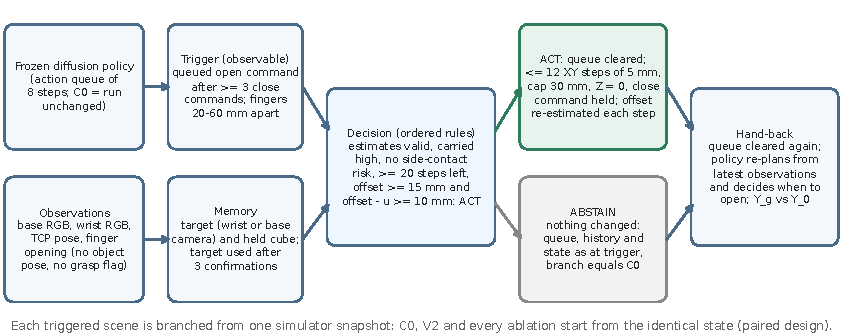
\includegraphics[width=\linewidth]{Fig02_method.pdf}
\caption{Vision-CENTER V2 as implemented. The trigger is an observable rule on the policy's own commands and the finger opening. At the trigger the controller combines current base- and wrist-camera estimates with a confirmed target memory and a held-cube memory. If it abstains, nothing is changed and the branch equals C0. If it acts, the policy's action queue is cleared, horizontal steps of at most 5\,mm are commanded with zero vertical command and the held close command, the offset is re-estimated after every step, and at the end the queue is cleared again so that the frozen policy re-plans from its latest observations. Every arm is branched from the same simulator snapshot.}\label{fig:method}
\end{figure}

\paragraph{Trigger} The trigger fires at the first control step at which three observable conditions hold: the gripper component of the policy's next queued action is an open command; the policy's last three or more executed gripper commands were close commands; and the finger opening (sum of the two finger joints) is between 0.02 and 0.06\,m, i.e.\ neither empty nor fully open. The rule does not read whether, or which, object is grasped. It can therefore fire when the fingers hold the wrong object: in development scene 51152 (policy seed 2) the policy had grasped the \emph{target} cube; every vision arm, including V2, abstained there for lack of a held-cube estimate, and only the privileged oracle moved (Section~\ref{sec:physics}). At the trigger the pending action has not yet been executed. If the controller abstains, the simulator state, the action queue, the observation history and the counters are left untouched (checked in every run), so the branch is identical to C0.

\paragraph{Observations} The controller receives the base and wrist RGB images ($128\times128$ each), the TCP pose, the finger opening and the last executed gripper command. Cubes are located by colour segmentation and projected with the fixed camera parameters; no model is trained.

\paragraph{Memory} The target cube is often hidden by the held cube at the trigger, so V2 keeps two memories, updated at every step from the start of the episode. The \emph{target memory} stores one position with a reading bound $u$: a step with an accepted wrist-camera fit ($u=2$\,mm) updates it, otherwise a step with an accepted base-camera estimate ($u=5$\,mm) does. An observation consistent with the stored position (distance at most the sum of the two bounds) increases its confirmation count, and the more precise source keeps the position; an inconsistent one replaces it and restarts the count. The memory is used only after $m=3$ confirmations, its bound grows by 5\,mm if the gripper passed close to it unobserved, and it is refused if the current image contradicts it. Its source is recorded as \emph{hand} or \emph{base} memory. The \emph{hold memory} stores the held cube's position relative to the gripper; it is refitted every fourth step while the gripper is commanded closed ($u=2$\,mm) and dropped when the finger opening changes by more than 1\,mm. At the trigger, an accepted estimate from the current frame is preferred, otherwise the memory is used.

\paragraph{Decision} Let $\hat{\mathbf{o}}=\hat{\mathbf{x}}_{\mathrm{target}}-\hat{\mathbf{x}}_{\mathrm{held}}$ be the estimated horizontal offset and $u$ the bound of the target estimate. The rules are evaluated in a fixed order and the first that applies decides: no held-cube estimate, no target estimate, or memory contradicted (abstain); held cube centre estimated below 58\,mm, or a remembered target with the held cube's bottom below the target's top face (\textsc{low carry}); offset at least 40\,mm (plus $u$ for a remembered target) with less than 3\,mm vertical clearance (\textsc{side-contact risk}); fewer than 20 steps left in the episode; $\|\hat{\mathbf{o}}\|<15$\,mm (\textsc{aligned}); $\|\hat{\mathbf{o}}\|-u<10$\,mm (\textsc{aligned within uncertainty}). Otherwise V2 acts, so acting requires
\begin{equation}
\|\hat{\mathbf{o}}\| \;\ge\; 15\ \mathrm{mm} \qquad\text{and}\qquad \|\hat{\mathbf{o}}\| - u \;\ge\; 10\ \mathrm{mm}.
\end{equation}

\paragraph{Bounded move} If V2 acts, it clears the policy's action queue (the pending open command is discarded) and, at each control step $t$, commands a horizontal TCP increment $\Delta\mathbf{x}_t$ towards the current offset estimate with
\begin{equation}
\|\Delta\mathbf{x}_t\|\le 5\ \mathrm{mm},\qquad \|\mathbf{x}_t+\Delta\mathbf{x}_t-\mathbf{x}_{t^\star}\|\le 30\ \mathrm{mm},\qquad t-t^\star< 12,
\end{equation}
where $\mathbf{x}_t$ is the measured TCP position and $\mathbf{x}_{t^\star}$ the TCP position at the trigger. The action sent to the end-effector delta-position controller has zero vertical component and repeats the last executed gripper command, which is a close command, so the grasp command is held rather than absent. No policy inference runs during the move (checked). After every step the images are read again and the offset is re-estimated, so the move is closed-loop on vision. It stops when the estimated residual is within 10\,mm (5\,mm when the target comes from memory), after 12 steps, at the target cap, at the end of the episode, or when the target estimate jumps by more than 3\,mm (plus $u$ for a remembered target), the estimate is lost, the held cube drops below 58\,mm, or the held cube shifts in the gripper by more than 3\,mm. Every step is charged to the 200-step episode budget.

\paragraph{Hand-back} At the end of the move the queue is cleared again. At the next step the frozen policy infers a new action chunk from its observation history, which now contains the observations made during the move; the policy decides when to open the gripper. In every acted V2 branch of all stages the policy re-planned at the first step after the move, and its first open command followed 1--24 steps later (median 2--3 by stage and policy); in one calibration branch it never opened the gripper again (Supplementary Table~S4).

\paragraph{Executed motion} The arm covered less than the commanded path: over all acted development branches, the net horizontal TCP displacement was 26--40\% of the commanded path length (medians 36\% and 37\% for the two policies), so 12 steps moved the TCP by roughly 20--25\,mm. This is an observed property of the controller in this simulator, not a bound. No V2 move ended at the 30\,mm cap; moves ended at the estimated tolerance or at the step budget. Offsets much larger than one move can remove are therefore only partly corrected (Section~\ref{sec:mechanism}).

\paragraph{Ablations and reference} \emph{V1} uses the wrist camera only and no memory. \emph{V2 single frame} gives V2 an empty memory until the trigger and lets it use only the trigger step's observation; because one frame cannot provide three confirmations, it accepts a single estimate ($m=1$), which favours this arm. \emph{V2 without hand / base / hold memory} prevents wrist-camera fits, base-camera estimates or held-cube fits from entering the memory. \emph{V2 rules off} keeps the full memory and removes, as one bundle, the three V2-specific rules (\textsc{aligned within uncertainty}, \textsc{side-contact risk}, and the \textsc{low carry} rule for a remembered target); the estimate-validity rules, the height rule, the step-budget rule and the 15\,mm rule inherited from V1 remain. \emph{Oracle centring} replaces the estimates by the true cube positions and is privileged.

%% ---------------------------------------------------------------------------------------------------------
\section{Experimental protocol}\label{sec:protocol}

\paragraph{Task and simulator} We use \texttt{StackCube-v1} of ManiSkill3 \cite{tao2024maniskill3} (version 3.0.1, commit \texttt{a4a4f92}) on SAPIEN 3.0.3 \cite{xiang2020sapien} with CPU PhysX, a single environment, a Panda arm with a wrist camera, end-effector delta-position control, and a 200-step horizon. Success is the first time the task condition holds (cube A on cube B, static, released); the episode then ends.

\paragraph{Frozen policies} The base policies are RGB diffusion policies \cite{chi2023diffusion} (observation horizon 2, prediction 16, execution 8) with an ImageNet-pretrained ResNet-18 encoder \cite{he2016resnet}, trained on the same 500 motion-planning demonstrations with two training seeds (\emph{policy seed 1} and \emph{policy seed 2}) and frozen before any intervention data were collected. The generalisation study uses a third frozen policy with the original small, non-pretrained convolutional encoder (\emph{PlainConv}).

\paragraph{Splits} Splits are disjoint ranges of scene seeds; all branches of a scene stay in one split.
\begin{itemize}
\item Development (C1): seeds 51100--51299, 200 scenes per policy, all arms.
\item Calibration: seeds 30000--30399, 400 scenes per policy, C0 and V2.
\item Final Test: seeds 90000--90399, 400 scenes per policy, C0 and V2, run once.
\item Generalisation (development level): seeds 51300--51499, PlainConv policy.
\end{itemize}
Before each stage, a placement check confirmed that no new scene repeats a cube placement of any earlier scene (0 identical placements among 2,347 references for calibration and for test).

\paragraph{Pre-registration and freezing} The development stage pre-registered two hypotheses: $H_{\mathrm{gen}}$ (V2 improves on C0 for policy seed 2, which was not used while developing V2) and $H_{\mathrm{mem}}$ (V2 improves on its single-frame variant for both policies, tested as an intersection--union test), with Holm over the two. The candidate (V2 with unchanged constants), the policy family, $\varepsilon$, $\delta$, the tests and all rules were then frozen in a manifest before calibration (SHA-256 \texttt{01b70a06\ldots}). The Final Test manifest (\texttt{94c5a591\ldots}) added the calibration analysis and the environment, and the test runner refused to start unless the live environment matched it (GPU, driver, Python version, upstream commit and the full package list) and three used development scenes reproduced bit for bit the reference recorded on the calibration host.

\paragraph{Hosts} Development ran on a host with NVIDIA driver 550.120. Calibration and the Final Test ran on RTX 4090 hosts with driver 595.99.02. Rendering differs between the two drivers, and with it some policy actions: in 16 of 300 earlier scenes and in 6 of 11 selected diagnostic scenes the outcome differed between hosts. The certificate and the test result therefore refer to the 595.99.02 configuration (Section~\ref{sec:limits}).

\paragraph{Policy sampling noise} The diffusion sampling noise is keyed to the scene and the control step, and is identical for all branches up to the trigger. After a move the policy resumes later and therefore draws different noise than C0 at the same phase of the task, so a discordant pair can reflect policy variance as well as the move. In an earlier development pilot, an arm that only held the robot still for a matched number of steps gave 1 rescue and 1 harm against C0 on 100 scenes; we read this as the approximate size of that floor, not as a correction. The efficacy test compares the deployed system (policy plus controller) with the policy alone and remains valid in this sense.

\paragraph{Role of the AI agent} Experiment orchestration on rented GPU hosts, analysis code, recounts and figure generation were carried out with an AI coding agent (Claude, Anthropic) under the author's direction. Every protocol decision taken during the runs is listed with its approval status in Supplementary Section~S9; the author takes responsibility for all of them.

\paragraph{Recount} All headline numbers were recomputed from the raw scene records, after checking the SHA-256 of every trajectory file, by two implementations (the project code and an independent hand-written count with SciPy); they agreed exactly (Supplementary Section~S8).


%% ---------------------------------------------------------------------------------------------------------
\section{Development results}\label{sec:dev}

\paragraph{Question} On development scenes, does V2 rescue failures without harming successes, and does its memory matter?

\begin{table}[!htbp]
\centering\footnotesize
\caption{Development stage (C1, seeds 51100--51299): successes of 200 scenes, rescues and harms against C0, and number of scenes in which the arm moved. The trigger fired in 195 (seed 1) and 191 (seed 2) scenes. For the oracle the column counts the scenes in which it entered its control loop (every trigger); it actually moved in 93 and 102.}\label{tab:dev}
\resizebox{\linewidth}{!}{\input{\tabdir T2_development_arms.tex}}
\end{table}

\begin{table}[!htbp]
\centering\footnotesize
\caption{Pre-registered development hypotheses (exact one-sided paired tests; Holm over the two hypotheses at $\alpha=0.05$, i.e.\ the smaller p-value is compared with 0.025 and the larger with 0.05; IU = intersection--union).}\label{tab:devtests}
\resizebox{\linewidth}{!}{\input{\tabdir T3_development_tests.tex}}
\end{table}

\paragraph{Evidence} Table~\ref{tab:dev} lists all nine arms. V2 raised success from 171 to 184 (14 rescues, 1 harm) for policy seed 1 and from 164 to 180 (16 rescues, 0 harms) for policy seed 2. The privileged oracle reached 185 and 184. Both pre-registered hypotheses were rejected (Table~\ref{tab:devtests}): V2 against C0 for policy seed 2 ($16$ vs $0$, $p=1.5\times10^{-5}$) and V2 against its single-frame variant for both policies (intersection--union $p=0.0078$).

\begin{figure}[!htbp]
\centering
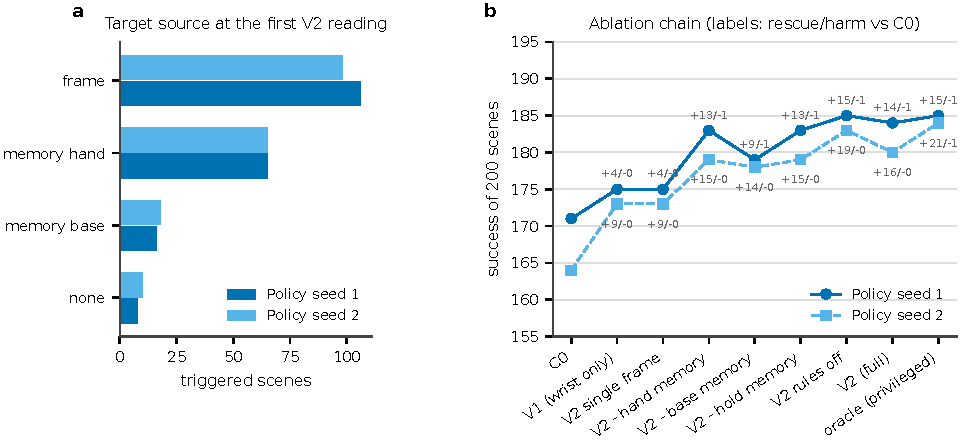
\includegraphics[width=\linewidth]{F4_memory_and_ablation.pdf}
\caption{Memory and ablation on the development scenes. (a) Source of the target estimate at the first V2 reading in triggered scenes: in about one third of them the target came from the wrist-camera memory, because the held cube hid it at the trigger. (b) Successes of all arms; labels give rescues/harms against C0. The single-frame variant behaves like the wrist-only V1, while removing one memory at a time loses less.}\label{fig:memory}
\end{figure}

\paragraph{Interpretation} Figure~\ref{fig:memory}a shows why memory matters: at the first reading the target position came from the current frame in 106 and 98 triggered scenes, from the hand memory in 65 and 65, and from the base memory in 16 and 18; in 8 and 10 there was no target estimate. Without confirmed memory (single frame) the controller acts in 25--30 scenes and rescues 4 and 9; with it, it acts in 39--41 scenes and rescues 14 and 16. Removing only the hand or the hold memory costs one rescue for seed 1 and one for seed 2, while removing the base memory costs five and two, which suggests that the memories partly substitute for each other.

\paragraph{Limits} The single-frame ablation sets the confirmation count to $m=1$, which also changes when a memory entry becomes usable; it is therefore not a pure removal of memory, and $H_{\mathrm{mem}}$ measures the combined effect (Section~\ref{sec:limits}). These are development results on scenes that informed the design; they do not certify a harm rate.


%% ---------------------------------------------------------------------------------------------------------
\section{Calibration certificate and Final Test}\label{sec:confirm}

\paragraph{Question} On new scenes and with nothing changed after development, can a conditional harm rate of 5\% or more be rejected (calibration), and does V2 increase success (Final Test)? The two questions are answered on disjoint scene sets with pre-registered tests; everything else in this section is labelled descriptive or post hoc.

\begin{figure}[!htbp]
\centering
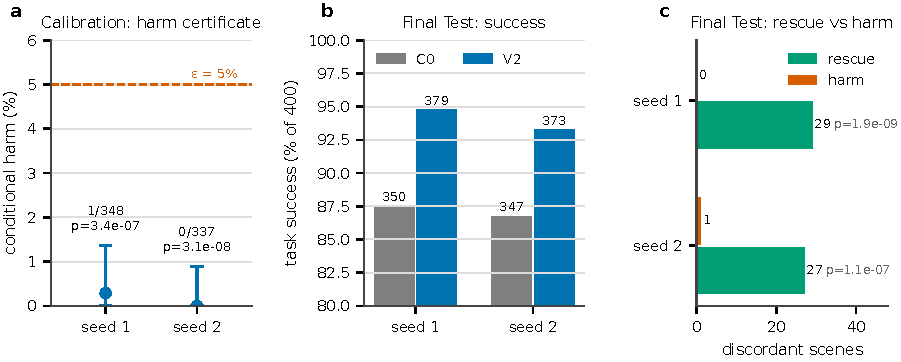
\includegraphics[width=\linewidth]{Fig04_statistics_calibration_vs_test.pdf}
\caption{Confirmatory stages, per policy. (a) Calibration (400 scenes per policy; harm counted among the $n_+$ baseline successes): observed conditional harm, its one-sided 95\% Clopper--Pearson upper bound (post hoc, descriptive) and the pre-registered level $\varepsilon=5\%$; p-values from Eq.~\eqref{eq:cert}, one-sided. (b) Final Test (400 held-out scenes per policy, run once): successes of C0 and V2. (c) Final Test discordant scenes and the one-sided p-values of Eq.~\eqref{eq:eff}.}\label{fig:stats}
\end{figure}

\begin{table}[!htbp]
\centering\footnotesize
\caption{Calibration certificate and Final Test. Trig.: scenes with a trigger; Acted: scenes in which V2 moved; C0, V2: successes of 400. Calibration tests $H_0: h(g)\ge 0.05$ (Eq.~\ref{eq:cert}); the Final Test tests efficacy (Eq.~\ref{eq:eff}); both with Holm over the two policies at level 0.05. Calibration success counts are descriptive.}\label{tab:confirm}
\resizebox{\linewidth}{!}{\input{\tabdir T4_calibration_and_test.tex}}
\end{table}

\paragraph{Evidence: calibration certificate} V2 turned 1 of 348 (policy seed 1) and 0 of 337 (policy seed 2) baseline successes into failures (Table~\ref{tab:confirm}, Fig.~\ref{fig:stats}a). The exact p-values were $3.4\times10^{-7}$ and $3.1\times10^{-8}$, below their Holm thresholds of 0.05 and 0.025, so both nulls $h(g)\ge0.05$ were rejected and both policies are certified at family-wise level $\delta=0.05$ (Section~\ref{sec:problem} states what this guarantees). As descriptive quantities, the one-sided 95\% Clopper--Pearson upper bounds \cite{clopper1934} of the conditional harm are 1.36\% and 0.89\%. The calibration success counts (348 to 371 and 337 to 366) were pre-declared as descriptive and are not used as evidence of efficacy.

\paragraph{What carries the certificate} Abstaining and untriggered branches equal C0 by construction, so harm can occur only where V2 moves. V2 moved in 73 and 66 calibration scenes, of which 48 and 36 were baseline successes; it caused 1 and 0 harms among them. Restricted to these scenes, the one-sided 95\% Clopper--Pearson upper bounds are 9.5\% and 8.0\% (post hoc; on the test split 0 of 38 and 1 of 46, bounds 7.6\% and 9.9\%). Most of the margin of the certificate therefore comes from abstention. The certificate is a statement about the deployed system, the policy together with its gated controller; it is not a bound on the harm of a move once V2 decides to act. The level $\varepsilon=5\%$ was fixed at the start of the project; it corresponds to about 17 lost successes out of 348, more than the 14 rescues observed for policy seed 1 in development.

\paragraph{Evidence: Final Test} The Final Test ran once, after a separate approval, with the frozen manifest verified before and after the run. Success rose from 350 to 379 (87.5\% to 94.75\%) for policy seed 1 and from 347 to 373 (86.75\% to 93.25\%) for policy seed 2. The discordant scenes were 29 rescues and 0 harms ($p=1.9\times10^{-9}$) and 27 rescues and 1 harm ($p=1.1\times10^{-7}$), so both efficacy nulls were rejected under Holm (Fig.~\ref{fig:stats}b,c). As a post hoc description, a paired bootstrap over scenes (20,000 resamples, percentile intervals) gives 95\% intervals for the success difference of $[+4.8, +10.0]$ and $[+4.0, +9.0]$ percentage points. Harm on the test scenes was 0 of 350 and 1 of 347; these counts are a descriptive re-observation, and the harm guarantee rests on the calibration certificate.

\paragraph{Interpretation} The gain and the low harm seen in development carried over to 1,600 new paired scenes without any change to the controller. Pooled over both policies, the Final Test cells were 696 both-succeed, 56 rescues, 1 harm and 47 both-fail scenes (Fig.~\ref{fig:problem}a); the pooling is descriptive and no test is based on it.

\paragraph{Limits} The guarantee concerns the scene distribution $\mathcal{D}$ of this task, the two policies, the sampling assumption of Section~\ref{sec:problem}, and the simulator configuration of the calibration host. Calibration and test did not reproduce development outcomes exactly because of the host difference; one pre-declared smoke criterion (bit-identity with the development records) was therefore not met (Section~\ref{sec:limits}).

%% ---------------------------------------------------------------------------------------------------------
\section{Mechanism: how a rescue and a harm happen}\label{sec:mechanism}

\paragraph{Question} Which steps of the chain observation $\to$ memory $\to$ decision $\to$ move $\to$ hand-back produce rescues, and where does harm enter? This section is descriptive and uses development records (driver 550.120); the cases were selected as stated and are not a random sample.

\paragraph{Rescue} In the typical rescue (Fig.~\ref{fig:problem}b; the first seed-1 rescue in scene order) the policy has carried the cube to a position beside the target and queued an open command there. V2 discards that command, moves the gripper towards the estimated target position, and hands back; the re-planned policy opens the gripper a few steps later (median 2--3 steps after the move in all stages) over the target, and the cube is placed.

\begin{figure}[!htbp]
\centering
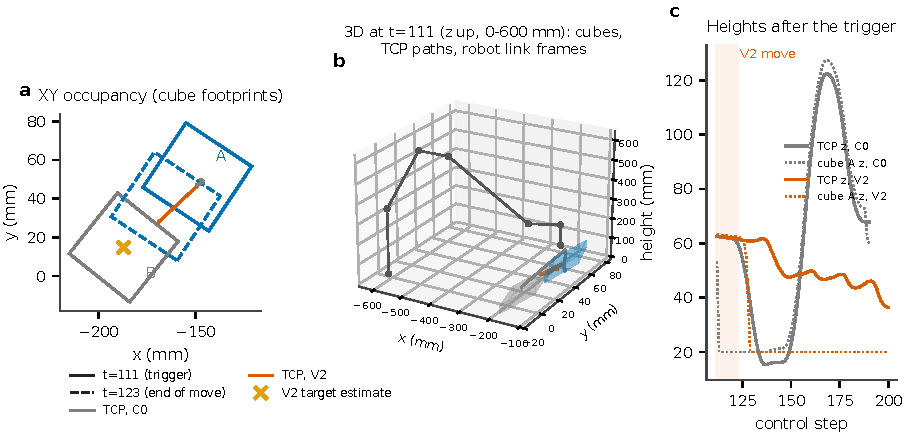
\includegraphics[width=\linewidth]{Fig05_spatial_51157.pdf}
\caption{The development harm case 51157 (policy seed 1; the only V2 harm for this policy in development). (a) Footprints of the held cube A (blue) and target cube B (grey) at the trigger (solid) and at the end of the V2 move (dashed), the TCP paths of C0 and V2 and the V2 target estimate, from the logged poses. (b) Three-dimensional view at the trigger: cube boxes from the logged poses, TCP paths of C0 (grey) and V2 (orange), and the robot link frames (origins, not collision meshes). (c) Heights of the TCP and of cube A after the trigger; the shaded band is the V2 move.}\label{fig:spatial}
\end{figure}

\paragraph{Harm} In scene 51157, the single development harm of V2 for policy seed 1, V2 did what it was designed to do. At the trigger the held cube was 54.6\,mm from the target centre; the V2 estimate was 54.7\,mm (error 0.15\,mm), within its 9\,mm reading bound. V2 moved for the full 12 steps; the TCP moved 24.3\,mm, and the true offset fell to 30.4\,mm (Fig.~\ref{fig:spatial}a). The move followed its commanded direction (cosine above 0.999 at every step, so this move passed Check 4) but not its commanded length: each 5\,mm command produced about 2\,mm of TCP displacement (Fig.~\ref{fig:control}a,b). Three steps after the hand-back the re-planned policy opened the gripper with the cube still beside the target; the cube fell to the table and the policy did not regrasp it before the horizon (Fig.~\ref{fig:spatial}c). Without V2 the policy also dropped the cube beside the target, but it regrasped it and completed the stack at step 190, 10 steps before the horizon; the 12 steps spent on the move exceed that margin. The record is consistent with two contributing factors, an incomplete correction and the time budget, and it does not separate them.

\paragraph{Offsets larger than one move} Acting on an offset that one move cannot remove is a weakness of the design. Among acted scenes with an estimated offset above 40\,mm there were 3 in development (1 rescue and 1 harm, the latter being 51157), none in calibration, and 8 in the Final Test (6 rescues and 1 harm, the only harm of the test).

\begin{figure}[!htbp]
\centering
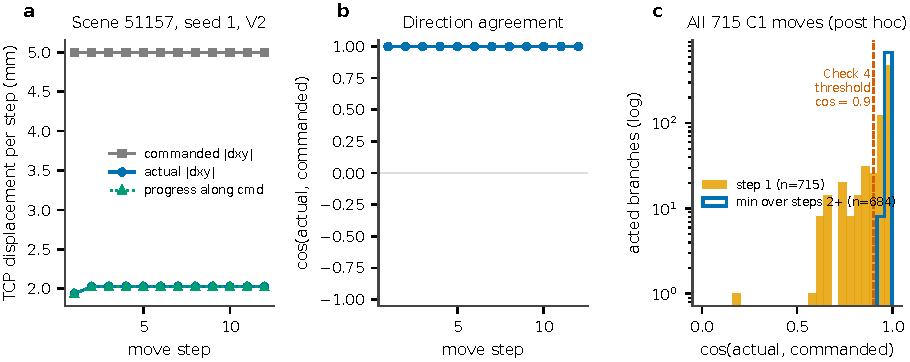
\includegraphics[width=\linewidth]{Fig06_control_check4.pdf}
\caption{Commanded versus executed motion. (a,b) Scene 51157, V2: commanded and executed horizontal TCP displacement per move step and their direction cosine. (c) All 715 acted development branches of all arms (post hoc): cosine between executed and commanded horizontal step, for the first step and for the minimum over steps 2 onwards (log scale). 110 branches fall below the pre-declared 0.9 threshold at the first step and none at later steps; the cause of the first-step deviation is not established.}\label{fig:control}
\end{figure}

\paragraph{The pre-declared motion check} Check 4 required, for every move step, a cosine of at least 0.9 between the executed and the commanded horizontal TCP step, and an executed step length of at least 0.2\,mm. It failed in 9 of 41 V2 moves for policy seed 1 and 5 of 39 for seed 2; we keep the official FAIL. In all 14 failures only the first step failed, and only on direction (cosine 0.63--0.88); the later steps of the same moves had cosine 0.934--0.999. Across all arms, 110 of 715 moves failed, all at the first step; a post hoc check of steps 2 onwards passed in all 715 (Fig.~\ref{fig:control}c). The failing V2 moves had a lower cosine between the first command and the TCP motion just before the trigger (median $-0.57$ against $0.66$ for passing moves), which is consistent with the arm still carrying the policy's previous motion; we did not log controller internals, so this association is not an established cause.

\paragraph{Missed rescues} The oracle rescued 15 and 21 development scenes; V2 rescued 14 and 16. Of the oracle rescues, V2 missed 1 (policy seed 1) and 5 (policy seed 2), all by abstaining: side-contact risk (2), held cube too low (2), no target estimate (1), and aligned within the reading bound (1). Supplementary Table~S3 lists the decisions of every stage.

\paragraph{Limits} The mechanism is descriptive, read from development records on driver 550.120, and is not a causal decomposition. Scene 51157 is one case; its C0 branch has a different outcome on the calibration host, so the case describes the development configuration rather than the certified one.

%% ---------------------------------------------------------------------------------------------------------
\section{Validity of the physical record}\label{sec:physics}

\paragraph{Question} The mechanism analysis uses logged contacts, distances and poses. Are these measurements trustworthy, and does any failure change a result?

\begin{table}[!htbp]
\centering\footnotesize
\caption{Measurement-validity checks on the development record (post hoc unless stated). S4--S6 were declared before the analysis; their official status is kept.}\label{tab:physics}
\input{\tabdir T5_physics_validity.tex}
\end{table}

\paragraph{Checks} We defined three checks before analysing the record (Table~\ref{tab:physics}). \emph{S4}: during a move, the minimum distance between robot geometry and the target cube stays positive. \emph{S5}: reconstructed penetrations between bodies do not exceed 1\,mm. \emph{S6}: for each contact pair listed by PhysX, the logged separation agrees with the gap we reconstruct from the logged poses and collision shapes within 1\,mm.

\paragraph{Evidence} S4 failed in one of 715 acted branches, an oracle branch ($-2.16$\,mm, policy seed 2, scene 51152), and in none of the V2 branches. S5 failed in two short events with fast-moving cubes (11 of 3,874 branch records: 400 trunks plus 9 arms in each of 386 triggered scene-runs). Replacing every logged collision mesh by its convex hull changed no S4 or S5 status (Fig.~\ref{fig:hull}). S6 \emph{failed}: 54,267 of 580,539 listed pair rows (9.3\%) disagreed by more than 1\,mm (Fig.~\ref{fig:s6}a).

\begin{figure}[!htbp]
\centering
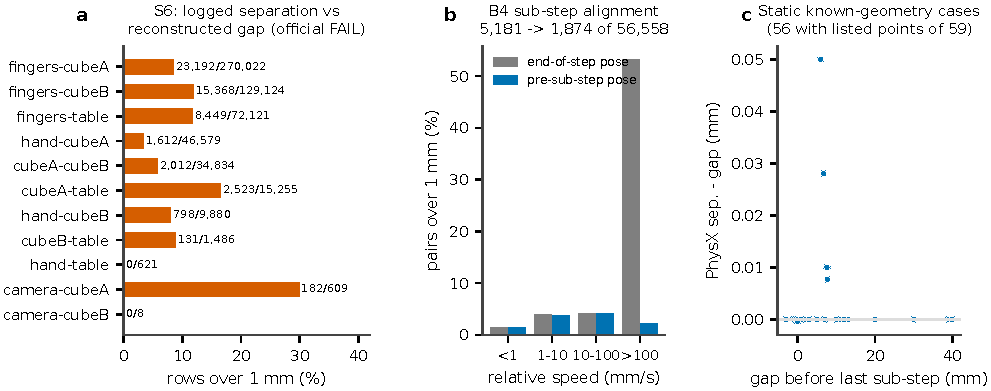
\includegraphics[width=\linewidth]{F7_physics_s6_b4.pdf}
\caption{Contact-separation check S6. (a) Rows over 1\,mm by pair kind (official FAIL). (b) Logging every physics sub-step on 11 used scene-runs: comparing with the pose before the last sub-step removes most disagreements of fast pairs. (c) Static boxes with known geometry: the PhysX separation equals the analytic gap before the last sub-step within 0.05\,mm.}\label{fig:s6}
\end{figure}

\paragraph{Partial explanation} Three follow-up measurements explain part of the S6 failure. First, on static box pairs with known geometry, the PhysX separation equals the analytic gap before the last sub-step within 0.05\,mm (Fig.~\ref{fig:s6}c), which fixes the definition of the logged quantity \cite{nvidia_physx_contact}. Second, logging every sub-step of 11 used scene-runs (re-run on the calibration host) showed that the contact list is computed at the pose before the last of the five sub-steps of a control step; comparing with that pose reduced the disagreements above 1\,mm from 5,181 to 1,874 of 56,558 pairs, and for pairs faster than 100\,mm/s from 3,436 to 146 (Fig.~\ref{fig:s6}b). Third, the remaining 1,874 rows are all zero-impulse proximity pairs between a finger box and a cube; shape-index mismatch and static edge geometry were excluded as causes. Their origin is not established.

\begin{figure}[!htbp]
\centering
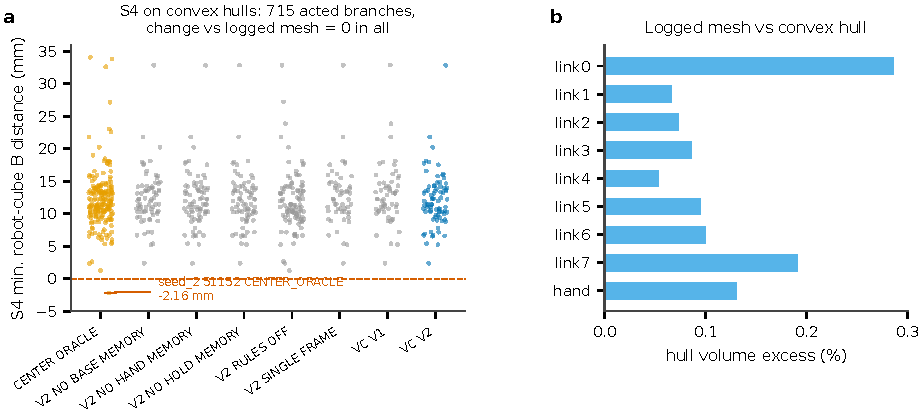
\includegraphics[width=\linewidth]{F8_hull_sensitivity.pdf}
\caption{Collision-geometry sensitivity. (a) S4 minimum robot--target distance on convex hulls for all 715 acted branches; the change with respect to the logged meshes is zero in every branch, and the only negative value is an oracle branch. (b) Volume excess of the convex hull over the logged mesh per link (at most 0.3\%).}\label{fig:hull}
\end{figure}

\paragraph{Interpretation} The task outcomes, the harm certificate and the efficacy test use only the success flag of each branch, which the simulator computes from its own state; they do not depend on S4--S6. The S6 failure limits the use of logged separations for fine-grained contact analysis, which is why we use them only descriptively.

\paragraph{Limits} S6 keeps its official FAIL status. No check here establishes continuous-time collision freedom; a contact between control steps can be missed.


%% ---------------------------------------------------------------------------------------------------------
\section{A second policy architecture}\label{sec:generalization}

\paragraph{Question} Is the gain specific to the two ResNet-18 policies, which share architecture and data and differ only in the training seed? This stage is development-level: one pre-declared test, no calibration.

\begin{figure}[!htbp]
\centering
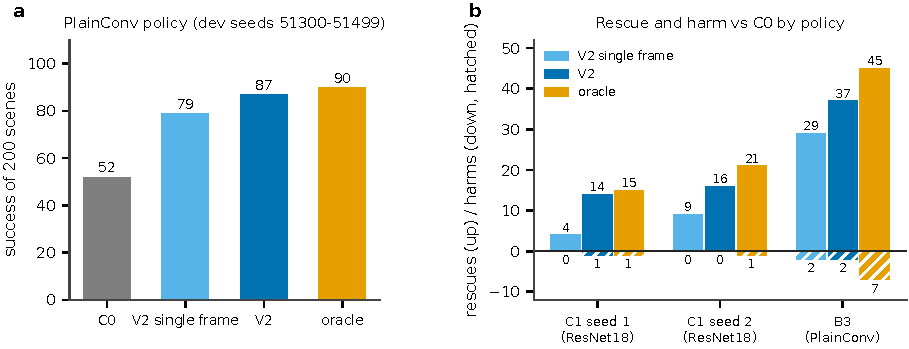
\includegraphics[width=\linewidth]{Fig09_generalization_plainconv.pdf}
\caption{Unchanged V2 on a frozen policy of a different architecture (PlainConv encoder; development seeds 51300--51499; same task and demonstrations). (a) Successes of 200 scenes. (b) Rescues (up) and harms (down, hatched) against C0 for the two ResNet-18 development policies and the PlainConv policy.}\label{fig:gen}
\end{figure}

\begin{table}[!htbp]
\centering\footnotesize
\caption{PlainConv policy, development level (200 scenes; two-sided 95\% Clopper--Pearson intervals, descriptive).}\label{tab:gen}
\input{\tabdir T6_generalization_plainconv.tex}
\end{table}

\paragraph{Evidence} Applied without any change to a frozen policy with a weaker, non-pretrained encoder, V2 raised success from 52 to 87 of 200 scenes, with 37 rescues and 2 harms ($p=1.4\times10^{-9}$, the single pre-declared test; Table~\ref{tab:gen}, Fig.~\ref{fig:gen}). It recovered 37 of the 45 oracle rescues; the oracle itself caused 7 harms. The single-frame variant reached 79 (29 rescues, 2 harms).

\paragraph{Interpretation and limits} The same release-time offset is a frequent failure of the weaker policy, and at development level V2 corrects many of these failures without retuning. There is no calibration certificate for this policy: its 2 harms among 52 baseline successes (3.8\%) are not a bound. The policies share the task and the demonstrations, so this is not evidence of transfer to other tasks.

%% ---------------------------------------------------------------------------------------------------------
\section{Discussion}\label{sec:discussion}

\paragraph{What the confirmatory results establish} Two pre-registered statements hold on new scenes: the conditional harm of the deployed system is below 5\% for both policies at family-wise error 0.05 (calibration), and the system succeeds more often than the policy alone for both policies (Final Test). Everything else in this paper, including the mechanism, the per-stage decisions, the bounds restricted to acting scenes and the bootstrap intervals, is descriptive or post hoc.

\paragraph{Separating rescue from harm changes what is reported} A success rate of 94.75\% against 87.5\% does not tell a user whether the intervention ever breaks a working episode. The paired four-cell count does: on the Final Test, 1 of 697 baseline successes was lost while 56 of 103 failures were rescued (pooled, descriptive). The certificate turns the calibration counterpart of this statement into a bound with a stated error probability, although most of its margin comes from scenes in which V2 does not move.

\paragraph{Abstention as a precaution, not a demonstrated cause} V2 acted in about one in five triggered scenes (41 of 195 and 39 of 191 in development). Most triggered scenes were already aligned, and in the rest V2 abstained when an estimate was missing, uncertain or contradicted. The rules-off ablation, which removes the three V2-specific rules as one bundle, acted in 53 and 50 development scenes instead of 41 and 39, gained one and three rescues, and had the same harms (1 and 0). The development data therefore do not show that these rules reduce harm, and the ablation cannot attribute any effect to a single rule. We kept the rules as a precaution before the confirmatory stages, and the certificate holds for the system with them.

\paragraph{Harm through time and incomplete motion} The observed development harm was not a collision but a combination of a move that covered less than its commanded path and a spent time budget. V2 already closes the loop on its own estimates after every step, but it does not check before acting whether the remaining offset can be removed within its step budget at the executed rate, nor whether the steps it spends leave the policy enough time. A feasibility gate based on the observed execution rate and the remaining horizon, or an estimate of the value of acting from earlier outcomes, are possible extensions; neither was implemented or tested.

\paragraph{What the memory does} Memory let V2 act when the target was hidden at the trigger. Because the ablation that removes earlier frames also lowers the confirmation count, our data support the statement that the confirmed multi-frame estimate improves on a single-frame estimate, not that memory alone does.

\paragraph{Wrong-object triggers} The trigger is an observable rule and can fire when the policy holds the wrong object, as in scene 51152. There V2 abstained for lack of a held-cube estimate, while the privileged oracle, which trusts the true cube positions, pushed the grasped target. Abstaining on missing estimates is therefore also a guard against a premise of the trigger that the robot cannot verify.

%% ---------------------------------------------------------------------------------------------------------
\section{Limitations}\label{sec:limits}

\begin{itemize}
\item \textbf{One task, simulation only.} All results are for \texttt{StackCube-v1} with rendered images. There is no real-robot experiment, and nothing is claimed about other tasks.
\item \textbf{Statistical, task-level guarantee.} The certificate controls the probability of certifying a system whose conditional harm is 5\% or more, under the assumption that calibration scenes are independent draws from the scene distribution and for the calibration host's simulator configuration. It is not a guarantee of physical safety, force limits or collision freedom, and most of its margin comes from abstention.
\item \textbf{Measurement validity.} The contact-separation check S6 failed (9.3\% of rows) and remains failed; in the sub-step re-run, 3.3\% of separated pairs remain unexplained.
\item \textbf{Host configuration.} Development ran on driver 550.120 and the confirmatory stages on driver 595.99.02. Outcomes differed between hosts in some scenes, so development estimates and the development mechanism analysis are linked to the confirmatory results only qualitatively.
\item \textbf{Deviation from a pre-declared criterion.} Before calibration, a smoke run was required to reproduce the development records bit for bit. It did not, because of the host difference; the runner did reproduce the unchanged development collector on the same host. The decision to proceed on a fixed host type was recorded and committed before the first calibration rollout by the AI agent that ran the experiment, without a prior approval by the author; the author reviewed it afterwards. It was not approved in advance. Nothing about the candidate, the policies, the levels or the tests changed.
\item \textbf{Ablation confounds.} The single-frame variant changes both the use of earlier frames and the confirmation count; the rules-off variant removes a bundle of three rules.
\item \textbf{No external baseline and policy-noise floor.} The comparators are the uninterrupted policy, ablations and a privileged oracle; no learned recovery or retry baseline was run. Part of the discordance may be policy variance after re-planning (Section~\ref{sec:protocol}).
\item \textbf{Two policies of one architecture} for the certificate (they differ only in the training seed), and a single PlainConv policy at development level.
\end{itemize}

%% ---------------------------------------------------------------------------------------------------------
\section{Conclusion}\label{sec:conclusion}

A recovery intervention on a frozen policy can rescue failures and can also destroy successes, and the two should be measured separately. With paired branching from a common snapshot, an exact binomial certificate on a calibration split and a single held-out confirmatory test, an observation-only release-time centring controller was certified (exact tests, family-wise error 0.05, calibration-host configuration) to have a conditional harm rate below 5\% for two diffusion policies, and it raised their success from 87.5\% to 94.75\% and from 86.75\% to 93.25\% on new scenes. Much of the harm margin comes from abstention, and the abstention rules were not shown to be the cause of the low harm. The descriptive mechanism analysis follows a representative rescue and the single development harm through the controller as implemented, including the re-planning hand-back and the shortfall between commanded and executed motion, and the audit of the physical record states which measurements can be trusted. The protocol can be applied to other recovery interventions; whether this controller transfers to other tasks or to a real robot remains open.

%% ---------------------------------------------------------------------------------------------------------
\section*{CRediT authorship contribution statement}
\textbf{[Author name to confirm]:} Conceptualization, Methodology, Software, Investigation, Formal analysis, Data curation, Visualization, Writing -- original draft, Writing -- review \& editing. [To be confirmed by the author.]

\section*{Declaration of competing interest}
[To be confirmed by the author.] The author declares that they have no known competing financial interests or personal relationships that could have appeared to influence the work reported in this paper.

\section*{Funding}
[To be confirmed by the author.] This research did not receive any specific grant from funding agencies in the public, commercial, or not-for-profit sectors.

\section*{Data availability}
[To be confirmed by the author.] The scene records, analysis code, figure and table generators, and SHA-256 manifests are available from the author's repository [link to be added]; raw trajectory archives (about 14\,GB) are available on request.

\section*{Declaration of generative AI and AI-assisted technologies in the manuscript preparation process}
[Draft; to be confirmed by the author.] During the preparation of this work the author used Claude (Anthropic) to write and run analysis code, draft text, and generate figures from the recorded data. After using this tool, the author reviewed and edited the content as needed and takes full responsibility for the content of the published article.



\bibliographystyle{elsarticle-num}
\bibliography{references}

\end{document}
